\documentclass[Ex4_Zusammenfassung.tex]{subfiles}

\begin{document}
\chapter{Bindungen \& Anregungen von Atomkernen}
Einleitend wollen wir direkt die Bethe--Weizsäcker--Formel für die Bindungsenergie von Atomen betrachten:

\begin{equation}
	m(Z,N) = Z m_H + N m_N - B(Z,N)
\end{equation}
wobei hier $m(Z,N)$ die Gesamtmasse, $Z$ die Protonen-- und $N$ die Neutronenzahl, $m_H$ die Masse des H--Atoms, $m_N$ die Masse eines Neutrons und $B(Z,N)$ die Bindungsenergie beschreiben.

\begin{figure}[h]
	\centering
	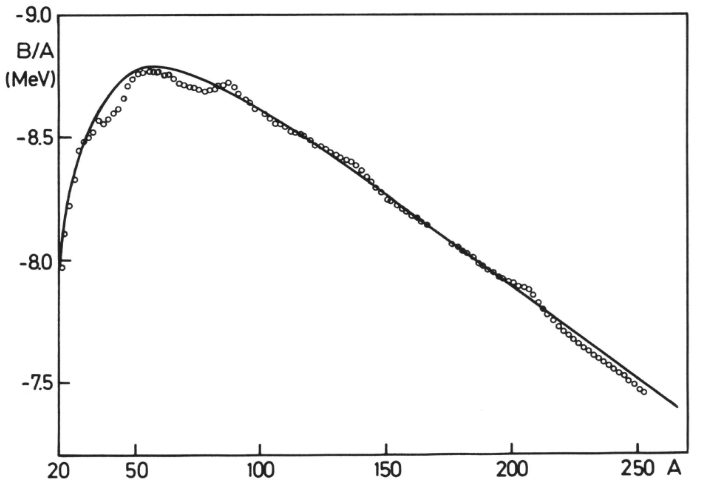
\includegraphics[scale=0.5]{bethe-weizsaecker.png}
	\caption{Kernbindungsenergie pro Nukleon im Vergleich zur Bethe--Weizsäcker--Formel. A ist hierbei die Anzahl der Nukleonen.}
\end{figure}

\section{Tröpfchenmodell}
Hierfür sei die Nukleonendichte eines Kerns konstant und sein Radius gegeben durch
\begin{equation}
	r = r_0 A^{\nicefrac{1}{3}}
\end{equation}
Beim Tröpfchen--Modell wird der Kern wie ein Tropfen einer inkompressiblen Flüssigkeit behandelt. Die Bindungsenergie ist gegeben durch
\begin{equation}
	B = B_1 + B_2 + B_3 + B_4 + B_5
\end{equation}
Die einzelnen Summanden wollen wir nun im Folgenden genauer betrachten:
\begin{enumerate}
	\item Volumenenergie: Kräfte, die bei der Vereinigung von Nukleonen frei werden. Proportional zur Anzahl der Nukleonen
		\begin{equation}
			B_1 = a_V A
		\end{equation}
	
	\item Oberflächenenergie: Nukleonen an der Oberfläche sind schwächer gebunden, da sie weniger Nachbarn besitzen
		\begin{equation}
			B_2 = a_S A^{\nicefrac{2}{3}}
		\end{equation}
	
	\item Coulomb--Energie: Abstoßung zwischen Protonen verringert die Bindungsenergie. Für eine homogen geladene Kugel $\propto \nicefrac{q^2}{r}$
		\begin{equation}
			B_3 = - a_C \frac{Z^2}{A^{\nicefrac{1}{3}}}
		\end{equation}
		
	\item Asymmetrie--Energie: Überschuss an Neutronen sorgt für höhere Besetzungszustände (Pauli--Prinzip) und die Bindung wird dadurch geringer (für $N=Z$ ist die Bindung maximal!)
		\begin{equation}
			B_4 = - a_A \frac{(N-Z)^2}{A}
		\end{equation}
		
	\item Paarungsenergie: Kerne mit geraden Protonen--/Neutronenzahlen sind stabiler (Im Schalenmodell haben solche Paare geringeren Spin!) 
		\begin{equation}
			B_5 = 
				\begin{cases}
					a_P A^{-\nicefrac{1}{2}} & \text{gerade Anzahl von $p$ und $n$}\\
					0 									   & \text{ungerade/gerade oder g./u. Anzahl von $p$/$n$}\\
					- a_P A^{-\nicefrac{1}{2}} & \text{ungerade Anzahl von $p$ und $n$}
				\end{cases}
		\end{equation}
	Das Schalenmodell ist ein Modell zum Aufbau der Atomkerne. Hierbei werden die Zustände nach dem Pauli--Prinzip \& der Drehimpulsquantisierung besetzt, ähnlich dem Modell für Elektronenschalen.
	 
	Allerdings:
		\begin{itemize}
			\item gibt es bei diesem Modell Protonen und Neutronen
			\item gibt es kein gemeinsames Kraftfeld (Protonen und Neutronen haben kurze Reichweite der starken Kernkraft und beeinflussen sich gegenseitig)
			\item ist die starke Kernkraft $\gg$ Coulomb--Kraft
		\end{itemize}
	Durch dieses Modell lassen sich die sogenannten \textbf{magischen Zahlen} beschreiben. Voll besetzte Schalen führen aufgrund kleinerem Spin zur stärkeren Bindung. Magische Zahlen sind demnach: 2, 8, 20, 28, 50, 82, 126, ... (aufgrund stärkerer Spin--Bahn--Kopplung etwas anders als für Elektronen). 
	
	Für magische Protonenzahlen gibt es viele stabile Isotope, für magische Neutronenzahlen viele stabile Isotone.
\end{enumerate}
Somit ergibt sich (wie oben schon erwähnt) die Gesamtbindungsenergie zu
\begin{equation}
	E_{\text{Binding}} = E_{\text{Volume}} - E_{\text{Surface}} - E_{\text{Coulomb}} - E_{\text{Asymmetry}} \pm E_{\text{Pairing}}
\end{equation}
Die einzelnen Komponenten sind in folgendem Bild sehr schön veranschaulicht
\begin{figure}[h]
	\centering
	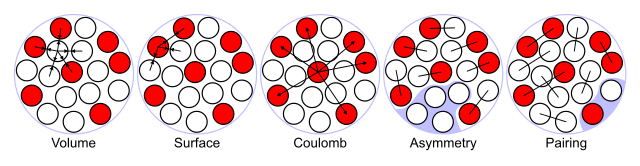
\includegraphics[scale=0.5]{liquid_drop.png}
	\caption{Visualisierung der verschiedenen Energie--Terme}
\end{figure}
Der Großteil des Periodensystems ist mit dieser Formel sehr exakt beschrieben. 

Bindungen im Vergleich zu $^{12}$C können durch ''Massenüberschuss'' ausgedrückt werden. 
\begin{equation}
	\Delta = M_{N,Z} c^2 - A\cdot \SI{931.502}{MeV}
\end{equation}

Für jedes Element existiert ein am stärksten gebundenes Isotop. Für kleine $Z$ ist die Form $N=Z$ ''bevorzugt''.
\begin{figure}[h]
	\centering
	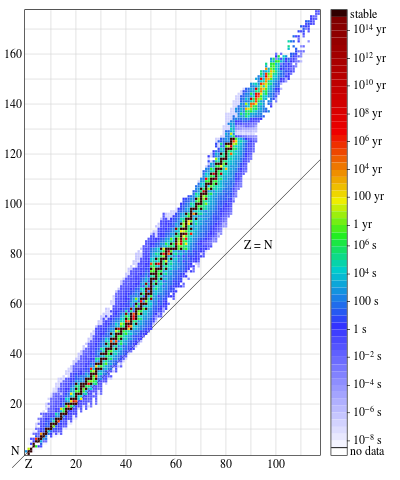
\includegraphics[width=0.58\textwidth]{isotopes.png}
	\caption{Halbwertszeiten der Isotope. Mit immer größer werdendem $Z$ weicht die Linie der stabilen Isotope immer weiter von der $N=Z$ Linie ab.}
\end{figure}
 Für große $Z$ hat Coulomb--Energie zunehmend Einfluss. $_{50}$Sn hat Isotope für $K=99-138$, 10 davon sind stabil, 30 radioaktiv mit hauptsächlichem $\beta^+$--Zerfall wenn $N$ zu klein ist, aber $\beta^-$--Zerfall wenn $N$ zu groß ist.
 
 Die Isotope sind eingeschlossen von der Protonen-- und Neutronendripline, außerhalb zerfallen die Kerne durch $p$ oder $n$ Emission in $\SI{E-18}{s}$. So gibt es bei schweren Kernen teilweise $\alpha$--Zerfall und jenseits von $^{208}$Pb $(Z=82,\ N=126)$ gibt es keine stabilen Kerne mehr.
 
 \subsubsection*{Wichtiger Punkt}
 Bei festen $A$ lässt sich die Masse als Funktion von $Z$ auftragen (Abb. \ref{massenparabel})
 \begin{figure}[h]
 	\centering
 	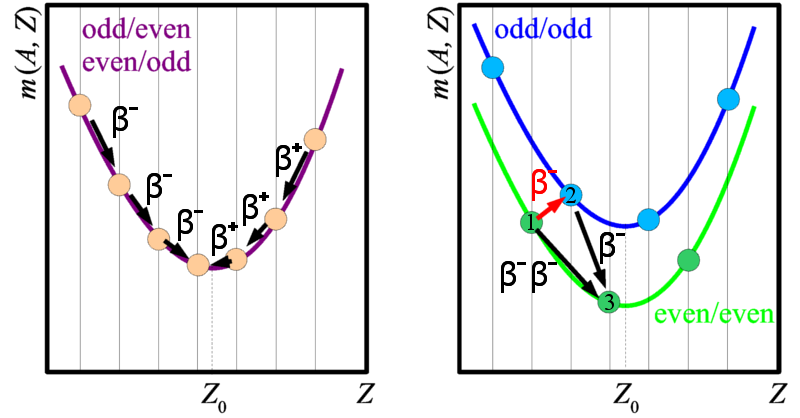
\includegraphics[scale=0.5]{Doppelbeta-massenparabel.png}
 	\caption{Massenparabel: hierbei ist quasi nur der geringste Energiezustand stabil.}
 	\label{massenparabel}
 \end{figure}
 Das Minimum lässt sich bestimmen durch: 
 \begin{equation}
 	Z_0(A) = \frac{A}{2} \lp \frac{m_N - m_H + a_A}{a_C A^{\nicefrac{2}{3}} + a_A} \rp 
 \end{equation}
 Die Werte für $Z_0$ ergeben die Linie größter Stabilität in der $N-Z$--Ebene.
 
 \section{Fermigasmodell}
 In diesem Modell sind die Nukleonen frei in einer Kugel mit Radius $r_0 A^{\nicefrac{1}{3}}$ (ohne Wechselwirkung), es gilt nur das Pauli--Prinzip. Wir wollen hier einmal die Potentialtöpfe der Protonen und Neutronen betrachten.
 \begin{figure}[H]
 	\centering
 	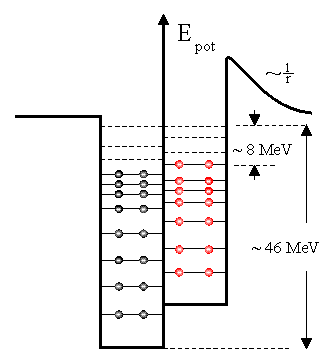
\includegraphics[scale=0.5]{potentialtopf_pn.png}
 	\caption{Der Potentialtopf eines Neutrons (links) bzw. eines Protons (rechts). n besetzte Niveaus}
 \end{figure}
 
 
\end{document}